\chapter{\glsentrylong{MPEG}}

\section{A collection of standards}
\begin{itemize}
\item Developed by the \gls{MPEG} (\href{https://www.itu.int}{ITU}),
  in 1992.
\item Define different algorithms to compress sequences of raster
  images (videos) and the corresponding audio.
\item All are lossy encoders.
\end{itemize}

\section{Versions}
\begin{enumerate}
\item \href{https://en.wikipedia.org/wiki/MPEG-1}{\textbf{MPEG-1}}
  (1993): Designed to store a movie in a \gls{CD} (\gls{VCD}).
\item \href{https://en.wikipedia.org/wiki/MPEG-2}{\textbf{MPEG-2}}
  (1996): Used in \glspl{DVD}, \href{https://en.wikipedia.org/wiki/Satellite_television}{satellite TV} and \href{https://en.wikipedia.org/wiki/Digital_television}{terrestial TV} (\gls{DVB}).
\item \href{https://en.wikipedia.org/wiki/MPEG-4}{\textbf{MPEG-4}}
  (1998): Used mainly in media streaming on the Internet.
\end{enumerate}

\section{Algorithm (1/2)}
\label{sec:MPEG-1_algo}
\begin{enumerate}
\item Convert to the \gls{YCbCr} color space, and
  \href{https://en.wikipedia.org/wiki/Chroma_subsampling}{subsample to
    4:2:0} (if the input is not yet in this format). /* Lossy */
\item Divide each channel in macro-blocks (MCs) of size 16x16. \popup{The
    rest of steps work by MCs}{This makes it possible to work
    at the MC level regardless of the image size.}.
\item \popup{Performing \gls{RDO}}{RDO implies that the video codec
    selects the optimal encoding decissions from a rate/distortion
    perspective. For example, if for the same quality (or distortion)
    a MB requires less bits if it is not motion compensated, then the
    codec does not compensate it. Thus, some MBs can be compensated
    while others not.},
  \href{https://en.wikipedia.org/wiki/Motion_compensation#Block_motion_compensation}{compensate
    the motion of each MC} using MCs of the \popup{adjacent
    images}{The MCs of the frame N, are compensated using the MCs of
    the frames N-1 and N+1.}. This step generates
  \popup{residue}{Residue MCs follow a Laplace distribution with mean
    0, and its entropy is smaller than the original MCs (this means
    that a residue MCs is more compressible than an original MC, on
    average).} MCs and a motion vector per MC, at
  \href{https://en.wikipedia.org/wiki/Motion_compensation}{half-pel
    accuracy}.
\item Divide each MC in 8x8 blocks.
\item Transform each block using the \gls{DCT}.
\item Quantize the \gls{DCT} coefficients. /* Lossy */
\item \popup{Entropy encode}{Using a combinatio of RLE and Huffman
    Coding (VLC = Variable Length Coding).} the quantized coefficients
  and the motion compensation data (motion vectors and reference
  frames).
\end{enumerate}

\section*{Algorithm (2/2)}
\begin{itemize}
\item A graphic description of a compression of a gray-scale sequence of images.
\end{itemize}
\vspace{-2ex}
\begin{center}
  \href{https://w3.ual.es/~vruiz/Docencia/Apuntes/Coding/Video/02-MPEG1/index.html}{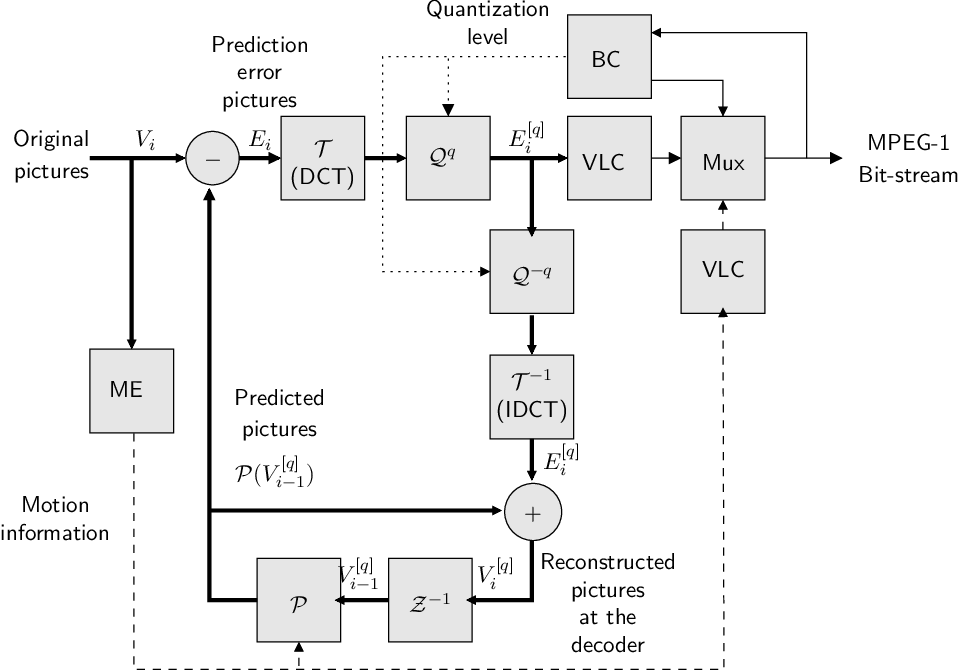
\includegraphics[width=8.5cm]{MPEG-1_compressor}}
\end{center}

\section{Blocking artifacts}
\begin{center}
  \href{https://filmora.wondershare.com/video-editing/video-compression-artifacts.html}{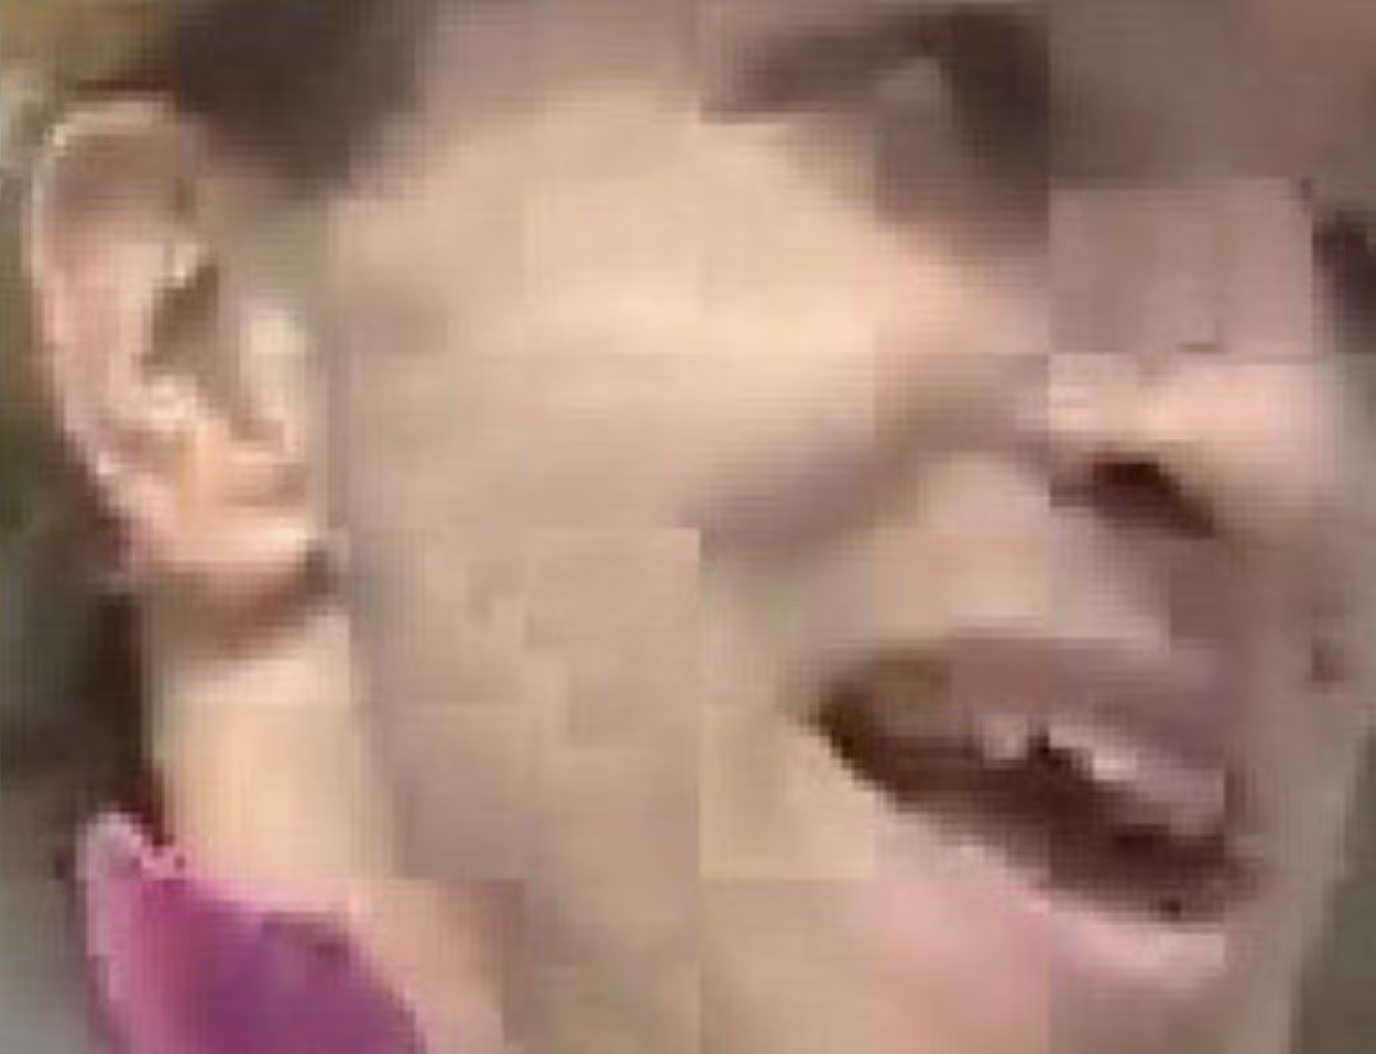
\includegraphics[width=8.5cm]{MPEG_artifacts}}
\end{center}
